%%%%%%%%%%%%%%%%%%%%%%%%%%%%%%%%%%%%%%%%%
% Beamer Presentation
% LaTeX Template
% Version 1.0 (10/11/12)
%
% This template has been downloaded from:
% http://www.LaTeXTemplates.com
%
% License:
% CC BY-NC-SA 3.0 (http://creativecommons.org/licenses/by-nc-sa/3.0/)
%
%%%%%%%%%%%%%%%%%%%%%%%%%%%%%%%%%%%%%%%%%

%----------------------------------------------------------------------------------------
%	PACKAGES AND THEMES
%----------------------------------------------------------------------------------------

\documentclass[c]{beamer}
%\documentclass[notes]{beamer}
\setbeamertemplate{note page}[show only notes]
\input{OR_common.tex}

% \usepackage{array}
% \newcolumntype{C}{@{}c@{}}
% \newcommand{\bottombox}[1]{\makebox[2em][r]{#1}\hspace*{\tabcolsep}\hspace*{2em}}%
% \newcommand{\innerbox}[2]{%
%     \begin{tabular}[b]{c|c}
%        \rule{2em}{0pt}\rule[-2ex]{0pt}{5ex} & \makebox[2em]{#2} \\\cline{2-2}
%        \multicolumn{2}{r}{{#1}\hspace*{1.5\tabcolsep}\hspace*{2em}\rule[-2ex]{0pt}{5ex}}
%     \end{tabular}}
% \renewcommand{\arraystretch}{1.25}

%%%%%%%%%%%%%%%%%%%%%%%%%%%%%%%%%%%%%%%%%%%%%%%%%%%%%%%%%%%%%%%%%%%%%%%%%%%%%
%%%%%%%%%%%%%%%%%%%%%%%%%%%%%%%%%%%%%%%%%%%%%%%%%%%%%%%%%%%%%%%%%%%%%%%%%%%%%
%%%%%%%%%%%%%%%%%%%%%%%%%%%%%%%%%%%%%%%%%%%%%%%%%%%%%%%%%%%%%%%%%%%%%%%%%%%%%

\title[Introduction]{Unit 5. Stochastic processes}

\author{Jordi Villà i Freixa}
\institute[FCT]{
Universitat de Vic - Universitat Central de Catalunya \\
Study Abroad. Operations Research\\
\medskip
\textit{jordi.villa@uvic.cat}
}
\date{7/01-16/5, 2022}
\logo{
\includegraphics[width=.1\textwidth]{../figures/FCT}}
\begin{document}

\begin{frame}
\titlepage
\end{frame}


\begin{frame}
    \frametitle{Preliminary}
    This course is strongly based on the monography on Operations Research by Carter, Price and Rabadi \cite{carter}, and in material obtained from different sources (quoted when needed through the slides).
\end{frame}

%%%%%%%%%%%%%%%%%%%%%%%%%%%%%%%%%%%%%%%%%%%%%%%%%%%%%%%%%%%%%%%%%%%%%%%%%%%%
%%%%%%%%%%%%%%%%%%%%%%%%%%%%%%%%%%%%%%%%%%%%%%%%%%%%%%%%%%%%%%%%%%%%%%%%%%%%%
%%%%%%%%%%%%%%%%%%%%%%%%%%%%%%%%%%%%%%%%%%%%%%%%%%%%%%%%%%%%%%%%%%%%%%%%%%%%%

\section{Markov chains}

\begin{frame}
\begin{Exercise}
    Here is a simple game:
\begin{itemize}
    \item a player bets on coin tosses, a dollar each time,
    \item the game ends either when the player has no money left
    or is up to five dollars.
\end{itemize}
If the player starts with three dollars, what is the chance that the game
    takes at least five flips?
    Twenty-five flips?
\end{Exercise}

At any point, this player has either \$0, or \$1, \ldots, or \$5.
We say that the player is in the
state
$s_0$, $s_1$, \ldots, or $s_5$.
A game consists of moving from state to state.
For instance,
a player now in state $s_3$ has on the next flip a $.5$ chance of moving
to state $s_2$ and a $.5$ chance of moving to $s_4$.
The boundary states are a bit different;
once in state~$s_0$ or state~$s_5$,
the player never leaves.

\end{frame}

\begin{frame}

Let $p_{i}(n)$ be the probability that the player is in state $s_i$
after $n$ flips.
Then, for instance, we have that the probability of being in state~$s_0$
after flip~$n+1$ is
$p_{0}(n+1)=p_{0}(n)+0.5\cdot p_{1}(n)$.
This matrix equation sumarizes.
\begin{equation*}
  \begin{pmatrix}
      1  &.5 &0  &0  &0   &0  \\
      0  &0  &.5 &0  &0   &0  \\
      0  &.5 &0  &.5 &0   &0  \\
      0  &0  &.5 &0  &.5  &0  \\
      0  &0  &0  &.5 &0   &0  \\
      0  &0  &0  &0  &.5  &1
   \end{pmatrix}
   \colvec{p_{0}(n) \\
        p_{1}(n) \\
        p_{2}(n) \\
        p_{3}(n) \\
        p_{4}(n) \\
        p_{5}(n)}
   =\colvec{p_{0}(n+1) \\
        p_{1}(n+1) \\
        p_{2}(n+1) \\
        p_{3}(n+1) \\
        p_{4}(n+1) \\
        p_{5}(n+1)}
\end{equation*}
\end{frame}

\begin{frame}
With the initial condition that the player starts with
three dollars, calculation gives this.
\begin{center}
  \begin{tabular}{@{}c|cccccc@{}}
    $n=0$
    &$n=1$
    &$n=2$
    &$n=3$
    &$n=4$
    &$\cdots$
    &$n=24$ \\
    \hline
    $\left(\begin{aligncolondecimal}{0}
             0 \\ 0    \\  0   \\  1    \\  0    \\  0
           \end{aligncolondecimal}
     \right)$
    &$\left(\begin{aligncolondecimal}{1}
       0      \\  0    \\  .5  \\  0    \\  .5    \\  0
             \end{aligncolondecimal}
     \right)$
    &$\left(\begin{aligncolondecimal}{2}
      0      \\  .25  \\ 0    \\ .5    \\  0     \\  .25
            \end{aligncolondecimal}
     \right)$
    &$\left(\begin{aligncolondecimal}{3}
        .125   \\   0   \\ .375 \\ 0     \\ .25    \\  .25
            \end{aligncolondecimal}
     \right)$
    &$\left(\begin{aligncolondecimal}{4}
        .125   \\ .1875 \\ 0    \\ .3125 \\ 0      \\ .375
            \end{aligncolondecimal}
     \right)$
    &$\cdots$
    &$\left(\begin{aligncolondecimal}{5}
        .39600 \\ .00276   \\ 0    \\ .00447 \\ 0  \\ .59676
            \end{aligncolondecimal}
     \right)$
  \end{tabular}
\end{center}
\end{frame}

\begin{frame}
\begin{itemize}
    \item The player quickly ends in either state~$s_0$
    or state~$s_5$. For instance, after the fourth flip there is a probability of $0.50$ that
    the game is already over: The boundary states
    are said to be {\bf absorbtive}.
    \item {\em The Markov chain model is
    historyless}: with a fixed transition matrix, the next state depends only on the current state,
    not on any prior states. More formally:
    \begin{eqnarray*}
    P(x_{t+1}=s_{t+1}|x_t=s_t, x_{t-1}=s_{t-1},...,x_1=s_1,x_0=s_0)=\\
    P(x_{t+1}=s_{t+1}|x_t=s_t)
  \end{eqnarray*}
    \item In addition, it is clear that the probability of a transition from state $i$ to state $j$ is independent of time ({\bf stationarity property}):
    \[
    P(x_{t+1}=j|x_t=i)=p_{ij}
    \]
    \item Each column vector is a probability vector (and it sums up 1) and the matrix is a transition matrix.
\end{itemize}
\end{frame}

\begin{frame}

\begin{Exercise}
    A study (\cite{MacdonaldRidge}, p.~202)
divided occupations in the United Kingdom into
upper level (executives and professionals),
middle level (supervisors and skilled manual workers),
and lower level (unskilled).
To determine
the mobility across these levels in a generation, about
two thousand men were asked, ``At which level are you,
and at which level was your father when you were fourteen years old?''
\end{Exercise}
\end{frame}

\begin{frame}
This equation and transition diagram summarizes the results.

  \begin{center}
\begin{equation*}
  \begin{pmatrix}
    T_{1,1}  &T_{1,2}  &T_{1,3}  \\
    T_{2,1}  &T_{2,2}  &T_{2,3}  \\
    T_{3,1}  &T_{3,2}  &T_{3,3}
  \end{pmatrix}^t
\rightarrow
    \begin{pmatrix}
      .60  &.29  &.16  \\
      .26  &.37  &.27  \\
      .14  &.34  &.57
    \end{pmatrix}
    \colvec{p_{U}(n) \\ p_{M}(n) \\ p_{L}(n)}
    =\colvec{p_{U}(n+1) \\ p_{M}(n+1) \\ p_{L}(n+1)}
  \end{equation*}
    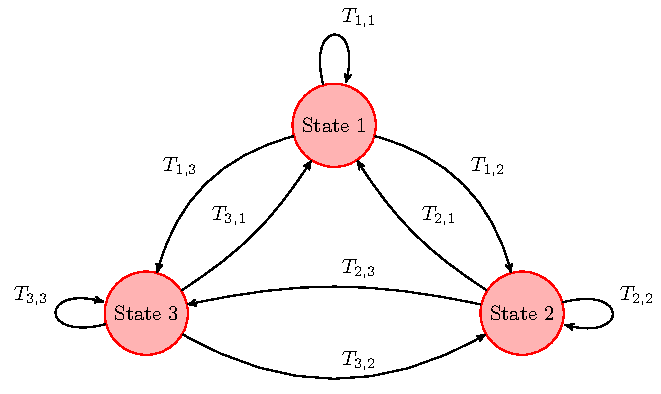
\includegraphics[width=0.7\linewidth]{../figures/transitiondiagram.pdf}
  \end{center}
\end{frame}

\begin{frame}
For instance,
a child of a lower class worker has a $.27$ probability of
growing up to be middle class.
Notice that the Markov model assumption about history
seems reasonable-- we expect that
while a parent's occupation has a direct influence on the occupation of the
child, the grandparent's occupation has no such direct influence.
With the initial distribution of the respondents's fathers given below,
this table lists the
distributions for the next five generations.
\begin{center}
  \begin{tabular}{c|ccccc}
    $n=0$  &$n=1$  &$n=2$  &$n=3$  &$n=4$  &$n=5$  \\ \hline
     $\left(\begin{aligncolondecimal}{2} .12 \\ .32  \\ .56 \end{aligncolondecimal} \right)$
    &$\left(\begin{aligncolondecimal}{2} .23 \\ .34  \\ .42 \end{aligncolondecimal} \right)$
    &$\left(\begin{aligncolondecimal}{2} .29 \\ .34  \\ .37 \end{aligncolondecimal} \right)$
    &$\left(\begin{aligncolondecimal}{2} .31 \\ .34  \\ .35 \end{aligncolondecimal} \right)$
    &$\left(\begin{aligncolondecimal}{2} .32 \\ .33  \\ .34 \end{aligncolondecimal} \right)$
    &$\left(\begin{aligncolondecimal}{2} .33 \\ .33  \\ .34 \end{aligncolondecimal} \right)$
  \end{tabular}
\end{center}
\end{frame}

\begin{frame}
\begin{Exercise}
The World Series of American baseball is
played between the team winning the American League
and the team winning the National League.
The series is won by the first team to win four games.
That means that a series is in one of twenty-four states:
0-0 (no games won yet by either team), 1-0
(one game won for the American League
team and no games for the National League team), etc.
If we assume that there is a probability $p$ that
the American League team wins each game then we have the following transition
matrix.
\end{Exercise}
\end{frame}

\begin{frame}
\begin{equation*}
  \begin{pmatrix}
    0      &0      &0      &0   &\ldots  \\
    p      &0      &0      &0   &\ldots  \\
    1-p    &0      &0      &0   &\ldots  \\
    0      &p      &0      &0   &\ldots  \\
    0      &1-p    &p      &0   &\ldots  \\
    0      &0      &1-p    &0   &\ldots  \\
    \vdots &\vdots &\vdots &\vdots
  \end{pmatrix}
  \colvec{p_{\text{0-0}}(n) \\ p_{\text{1-0}}(n) \\ p_{\text{0-1}}(n) \\
           p_{\text{2-0}}(n) \\ p_{\text{1-1}}(n) \\ p_{\text{0-2}}(n) \\
  \vdots }
  =
  \colvec{p_{\text{0-0}}(n+1) \\ p_{\text{1-0}}(n+1) \\ p_{\text{0-1}}(n+1) \\
           p_{\text{2-0}}(n+1) \\ p_{\text{1-1}}(n+1) \\ p_{\text{0-2}}(n+1) \\
           \vdots }
\end{equation*}
An especially interesting special case is $p=0.50$; this table lists the
resulting components of the $n=0$ through $n=7$ vectors. Check what happens with other values of $p$.
\end{frame}

\begin{frame}

\begin{center}\small
    \resizebox*{!}{0.8\textheight}{
\begin{tabular}{@{}rl|lllllll@{}}
      &$n=0$  &$n=1$  &$n=2$  &$n=3$  &$n=4$  &$n=5$  &$n=6$  &$n=7$  \\ \hline
  $\begin{array}{@{}c@{}}
    0-0 \\
    1-0 \\
    0-1 \\
    2-0 \\
    1-1 \\
    0-2 \\
    3-0 \\
    2-1 \\
    1-2 \\
    0-3 \\
    4-0 \\
    3-1 \\
    2-2 \\
    1-3 \\
    0-4 \\
    4-1 \\
    3-2 \\
    2-3 \\
    1-4 \\
    4-2 \\
    3-3 \\
    2-4 \\
    4-3 \\
    3-4
  \end{array}$
  &$\begin{aligncolondecimal}{0}
     1 \\
     0 \\
     0 \\
     0 \\
     0 \\
     0 \\
     0 \\
     0 \\
     0 \\
     0 \\
     0 \\
     0 \\
     0 \\
     0 \\
     0 \\
     0 \\
     0 \\
     0 \\
     0 \\
     0 \\
     0 \\
     0 \\
     0 \\
     0
   \end{aligncolondecimal}$
  &$\begin{aligncolondecimal}{1}
        0           \\
        0.5         \\
        0.5         \\
        0           \\
        0           \\
        0           \\
        0           \\
        0           \\
        0           \\
        0           \\
        0           \\
        0           \\
        0           \\
        0           \\
        0           \\
        0           \\
        0           \\
        0           \\
        0           \\
        0           \\
        0           \\
        0           \\
        0           \\
        0
   \end{aligncolondecimal}$
  &$\begin{aligncolondecimal}{2}
        0           \\
        0           \\
        0           \\
        0.25        \\
        0.5         \\
        0.25        \\
        0           \\
        0           \\
        0           \\
        0           \\
        0           \\
        0           \\
        0           \\
        0           \\
        0           \\
        0           \\
        0           \\
        0           \\
        0           \\
        0           \\
        0           \\
        0           \\
        0           \\
        0
   \end{aligncolondecimal}$
  &$\begin{aligncolondecimal}{3}
        0            \\
        0            \\
        0            \\
        0            \\
        0            \\
        0            \\
        0.125        \\
        0.375        \\
        0.375        \\
        0.125        \\
        0            \\
        0            \\
        0            \\
        0            \\
        0            \\
        0            \\
        0            \\
        0            \\
        0            \\
        0            \\
        0            \\
        0            \\
        0            \\
        0
   \end{aligncolondecimal}$
  &$\begin{aligncolondecimal}{4}
        0              \\
        0              \\
        0              \\
        0              \\
        0              \\
        0              \\
        0              \\
        0              \\
        0              \\
        0              \\
        0.0625         \\
        0.25           \\
        0.375          \\
        0.25           \\
        0.0625         \\
        0              \\
        0              \\
        0              \\
        0              \\
        0              \\
        0              \\
        0              \\
        0              \\
        0
   \end{aligncolondecimal}$
  &$\begin{aligncolondecimal}{4}
        0              \\
        0              \\
        0              \\
        0              \\
        0              \\
        0              \\
        0              \\
        0              \\
        0              \\
        0              \\
        0.0625         \\
        0              \\
        0              \\
        0              \\
        0.0625         \\
        0.125          \\
        0.3125         \\
        0.3125         \\
        0.125          \\
        0              \\
        0              \\
        0              \\
        0              \\
        0
   \end{aligncolondecimal}$
  &$\begin{aligncolondecimal}{5}
        0               \\
        0               \\
        0               \\
        0               \\
        0               \\
        0               \\
        0               \\
        0               \\
        0               \\
        0               \\
        0.0625          \\
        0               \\
        0               \\
        0               \\
        0.0625          \\
        0.125           \\
        0               \\
        0               \\
        0.125           \\
        0.15625         \\
        0.3125          \\
        0.15625         \\
        0               \\
        0
   \end{aligncolondecimal}$
  &$\begin{aligncolondecimal}{5}
        0             \\
        0             \\
        0             \\
        0             \\
        0             \\
        0             \\
        0             \\
        0             \\
        0             \\
        0             \\
        0.0625        \\
        0             \\
        0             \\
        0             \\
        0.0625        \\
        0.125         \\
        0             \\
        0             \\
        0.125         \\
        0.15625       \\
        0             \\
        0.15625       \\
        0.15625       \\
        0.15625
   \end{aligncolondecimal}$
\end{tabular}}
\end{center}

Evenly-matched teams are likely to have a long series-- there
is a probability of $0.625$ that the series goes at least six games.
\end{frame}

\begin{frame}
  In summary, a system can be modeled as a Markov process if it has the following four properties:
  \begin{itemize}
    \item Property 1: A finite number of states can be used to describe the dynamic behavior of the system.
    \item Property 2: Initial probabilities are specified for the system.
    \item Property 3: Markov property—We assume that a transition to a new state depends only on the current state and not on past conditions.
    \item Property 4: Stationarity property—The probability of a transition between any two states does not vary in time.
  \end{itemize}

\end{frame}

\begin{frame}
  If  Markov analysis is appropriate for the system being studiedone can try answering questions like:
\begin{itemize}
  \item How many transitions (steps) will it likely take for the system to move from some specified state to another specified state?
  \item What is the probability that it will take some given number of steps to go from one specified state to another?
  \item In the long run, which state is occupied by the system most frequently?
  \item Over a long period of time, what fraction of the time does the system occupy each of the possible states?
  \item Will the system continue indefinitely to move among all $N$ states, or will it eventually settle into a certain few states?
\end{itemize}
\end{frame}

\note{dynamic programming: https://www.youtube.com/watch?v=jqyfhFziDjw

https://www.techiedelight.com/word-break-problem/
}

\section{Hidden Markov Models}


\begin{frame}{Hidden Markov Models}
  HMMs are probably the most popular directed graphical model out there. They are used in many sequential and temporal domains:
  \begin{itemize}
    \item speech recognition,
    \item handwriting recognition,
    \item visual target tracking and localization,
    \item machine translation,
    \item robot localization,
    \item gene prediction,
    \item time-series analysis,
    \item natural language processing and part-of-speech recognition,
    \item stochastic control,
    \item protein folding, ...
  \end{itemize}
\end{frame}

\begin{frame}
  In HMMs, the random variables are divided into hidden states (phonemes, letters, target location) and observations (audio signal, pen strokes, target image). The goal is to predict the states from observations.

  What is this?
\begin{center}
  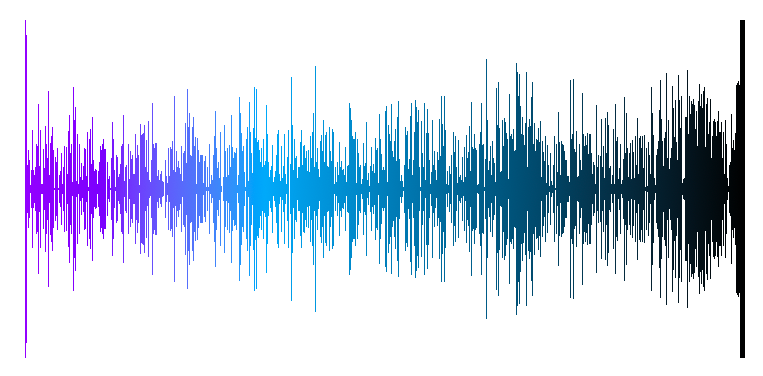
\includegraphics[width=0.7\linewidth]{../figures/SultansofSwing.png}
\end{center}
\end{frame}

\begin{frame}
We can start wth the graphical representation of the HMM
\begin{center}
 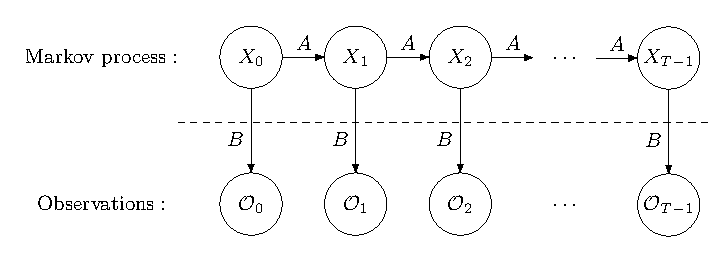
\includegraphics[width=0.7\linewidth]{../figures/HMM.pdf}
\end{center}
\end{frame}

% \begin{frame}
% To learn more on HMM:
% \begin{itemize}
%   \item \url{https://alliance.seas.upenn.edu/~cis520/wiki/index.php?n=Lectures.HMMs#toc7}
%   \item \url{http://www.columbia.edu/~mh2078/MachineLearningORFE/HMMs_MasterSlides.pdf}
% \end{itemize}
% \begin{frame}

\section{Discrete Evenet Simulations (DES)}
\begin{frame}{Running simulations in OR}
  \begin{center}
    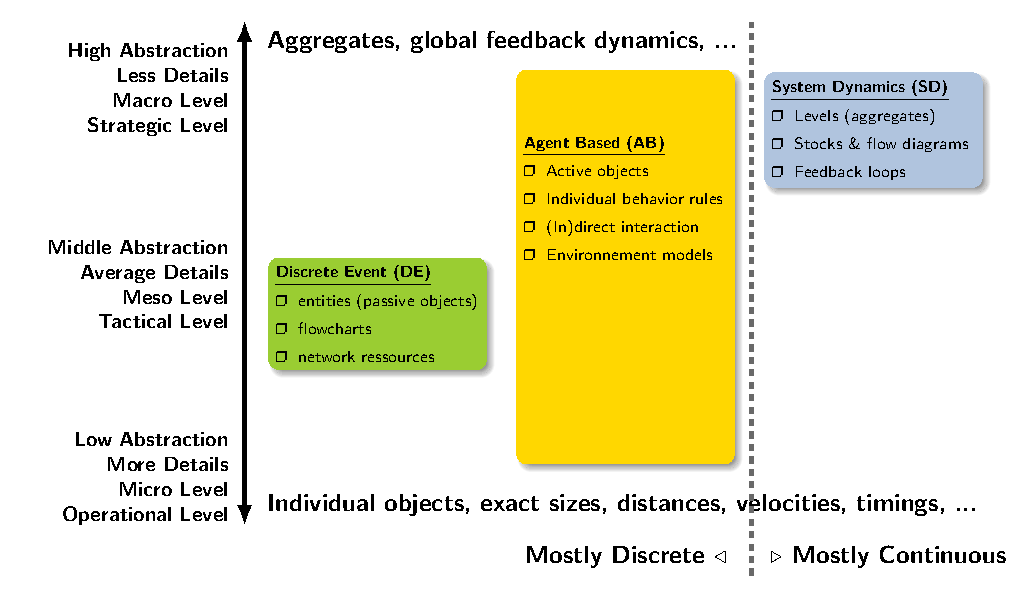
\includegraphics[width=0.7\linewidth]{../figures/simulation.pdf}
  \end{center}
  Taken from \url{https://texample.net/tikz/examples/simulation-abstraction/}
\end{frame}

\section{References}
\begin{frame}{References}
    \footnotesize
    \begin{thebibliography}{99}
    \setbeamertemplate{bibliography item}[text]
      \begin{columns}[t]
        \begin{column}{.45\textwidth}
            \bibitem{carter} Michael W. Carter, Camille C. Price, and Ghaith Rabadi. Operations Research, 2nd Edition. CRC Press.
            \bibitem{harel} David Harel, with Yishai Feldman. Algorithmics: the spirit of computing, 3rd Edition. Addison-Wesley.
            \bibitem{rardin} Ronald L. Rardin. Optimization in Operations Research, 2nd Edition. Pearson.
            \bibitem{hefferon} J. Hefferon. \href{http://joshua.smcvt.edu/linearalgebra}{Linear algebra (4th Ed)}.
        \end{column}
        \begin{column}{.45\textwidth}
            \bibitem{riley} K.F. Riley, M.P. Hobson, S.J. Bence. Mathematical Methods for Physics and Engineering (2nd Ed). McGraw Hill.
            \bibitem{nocedal} J. Nocedal, S. J. Wright. Numerical Optimization (2nd Ed). Springer.
            \bibitem{beers} Kenneth J. Beers. Numerical methods for chemical engineering: applications in Matlab. Cambridge University Press.
            \bibitem{barber} D. Barber. Bayesian reasoning and machine learning. Cambridge University Press.
        \end{column}
      \end{columns}
    \end{thebibliography}
\end{frame}
%----------------------------------------------------------------------------------------

\end{document}
